\chapter{Desarrollo de la Solución}
\label{sec:desarrollo}

\section[Proceso de Desarrollo]{Proceso de Desarrollo}

\subsection{Versionado de código}

\subsection{Integración Continua}

\subsection{Tests}

\section[Núcleo]{Núcleo}

El núcleo se encarga de administrar los datos no sensibles de los alumnos y sus materias cursadas, las inscripciones, planes de estudio con sus créditos, recorrido obligatorio y recomendado de inscripciones, etc.
El núcleo tiene la capacidad de servir dichos datos para que sean consumidos por los usuarios que tengan los permisos correspondientes.
Los usuarios tienen permisos asignados que corresponden con la carrera a la que pertenecen, que les permiten consultar datos de dicha carrera. 

### Alta, baja y modificación de datos
Los datos pueden ser creados, modificados y eliminados mediante una interfaz de Administrador. Asimismo, el núcleo consta de diferentes importadores para facilitar la carga.
Éstos importadores son:
- Carreras
- Planes de estudio con sus materias
- Prerrequisitos obligatorios y recomendados de materias
- Alumnos con sus datos personales
- Materias cursadas por alumnos
- Inscripciones a materias


\begin{figure}[h!]
  \centering
    
\includegraphics[scale=0.5]{images/nucleo/nucleo-fondoblanco.png}
  \captionof{figure}{Logo del Núcleo}
  \label{fig:django}
\end{figure}

\subsection{Tecnologías}

\subsection{API REST}

\subsection{Administración de los datos}

\subsubsection{Usuarios y permisos}

\subsubsection{Importadores}

\subsection{Pantallas principales}

\subsubsection{Login}
\begin{figure}[h!]
  \centering
    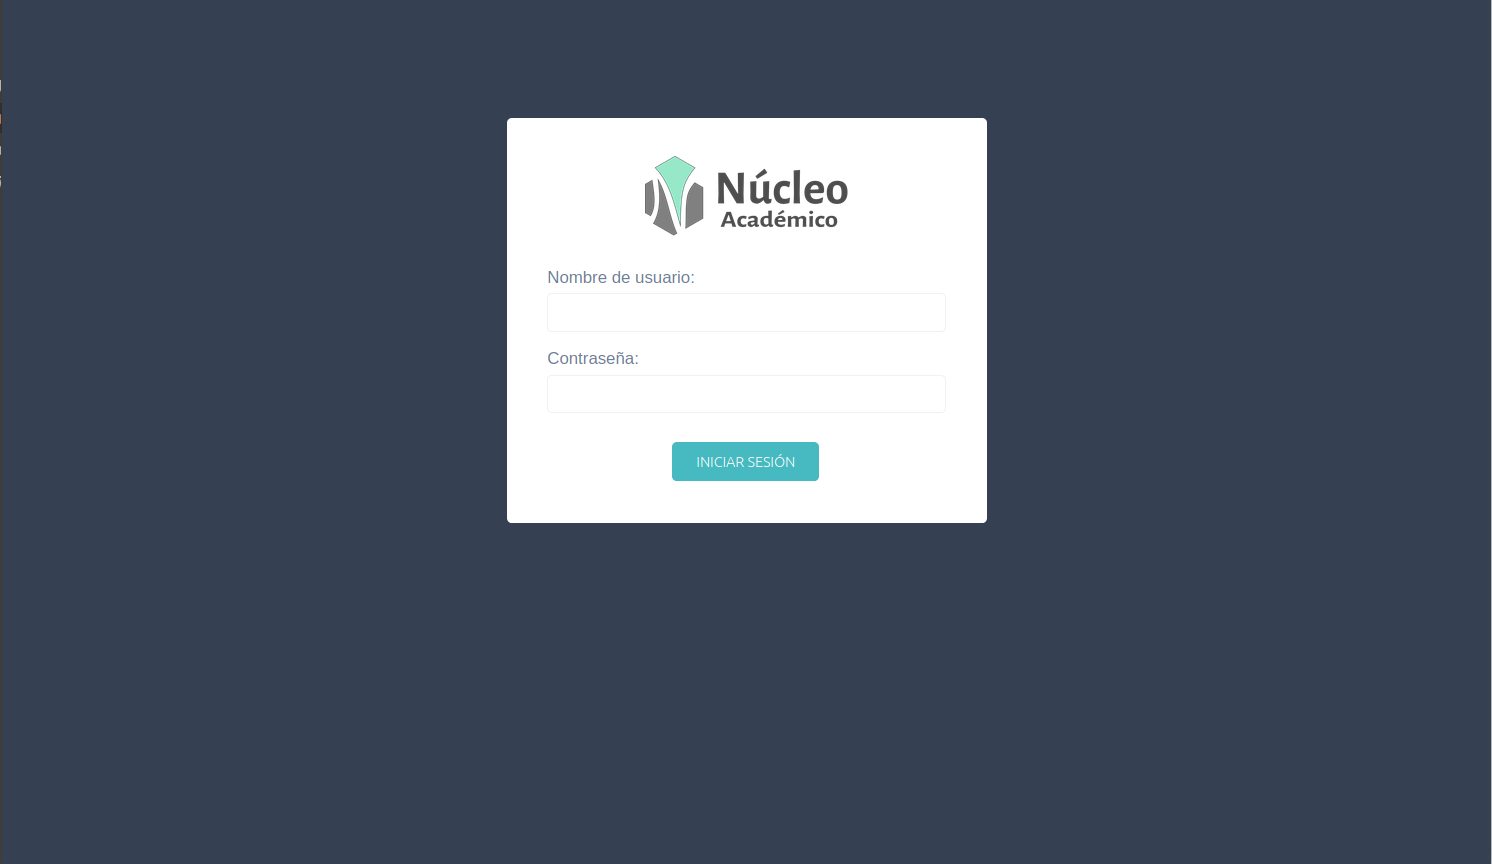
\includegraphics[scale=0.3]{images/nucleo/nucleo-login.png}
  \captionof{figure}{Pantalla de login}
  \label{fig:django}
\end{figure}

\subsubsection{Home}
\begin{figure}[h!]
  \centering
    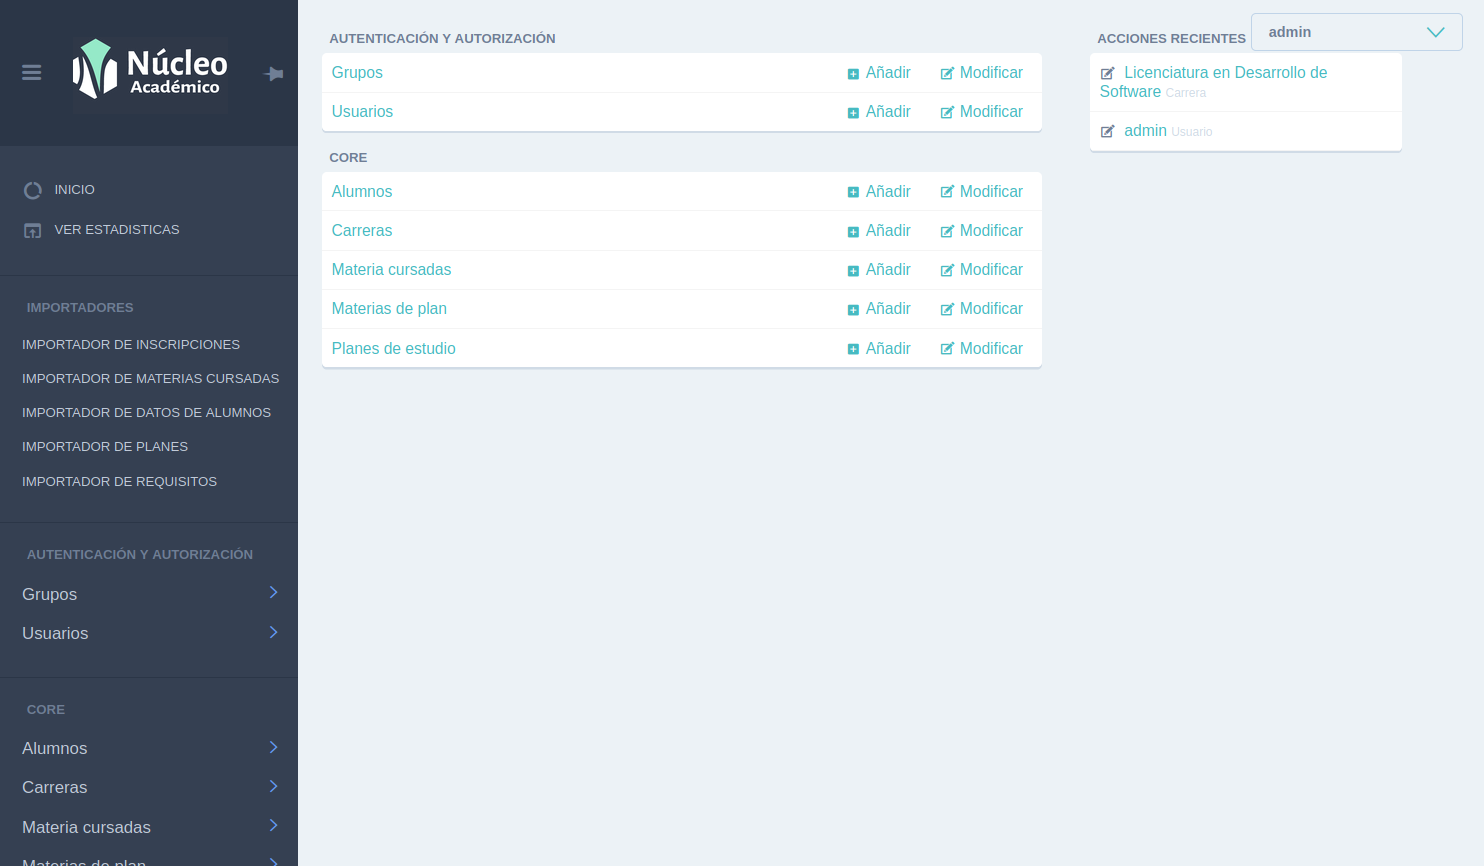
\includegraphics[scale=0.3]{images/nucleo/nucleo-home.png}
  \captionof{figure}{Pantalla de login}
  \label{fig:django}
\end{figure}

\subsubsection{Importadores}
\begin{figure}[h!]
  \centering
    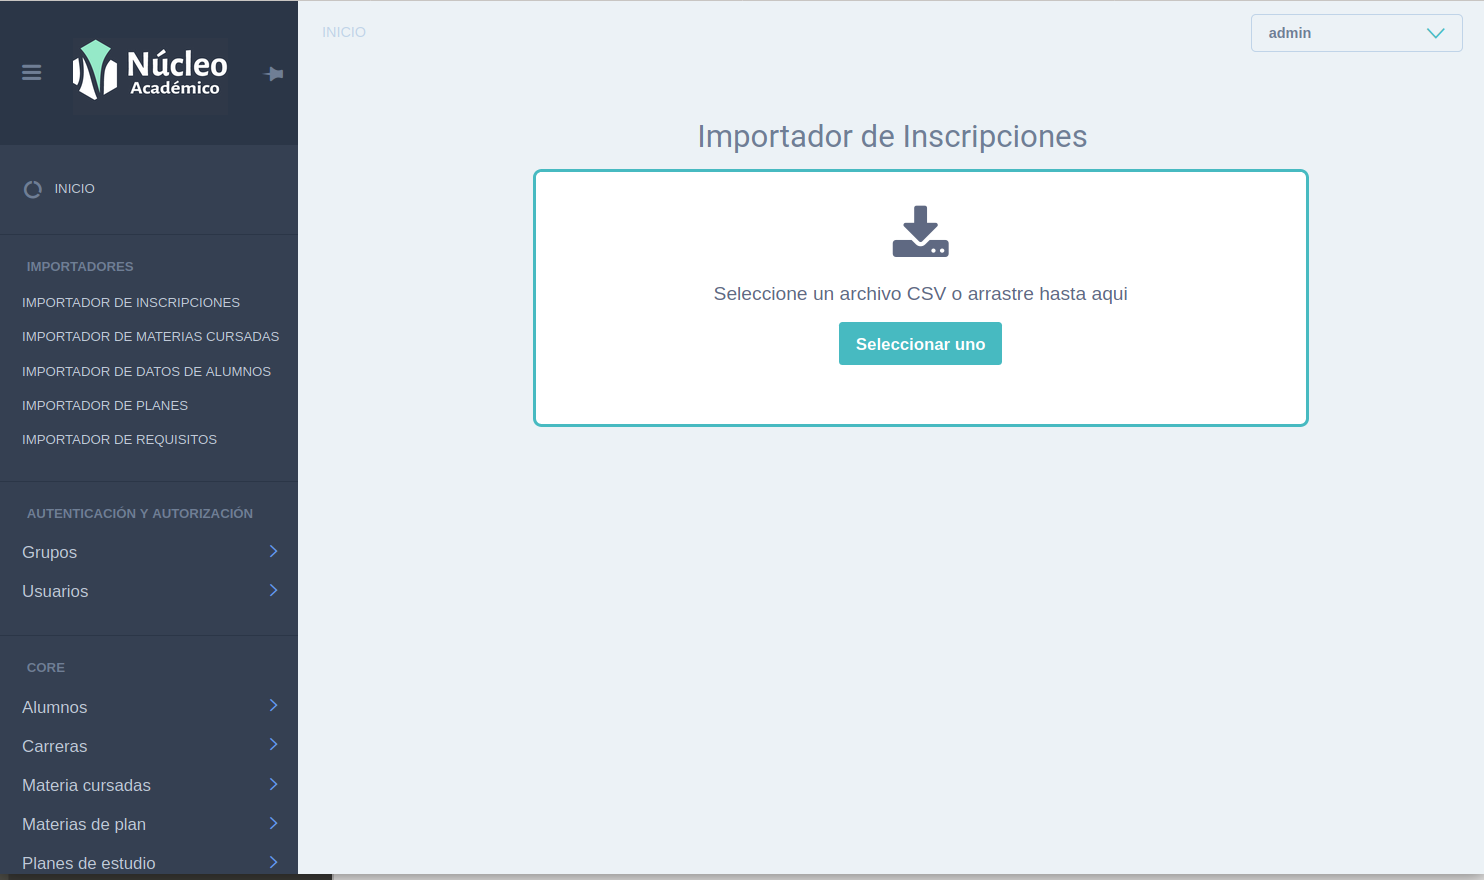
\includegraphics[scale=0.3]{images/nucleo/nucleo-importador.png}
  \captionof{figure}{Pantalla de login}
  \label{fig:django}
\end{figure}

\subsubsection{Listado}
\begin{figure}[h!]
  \centering
    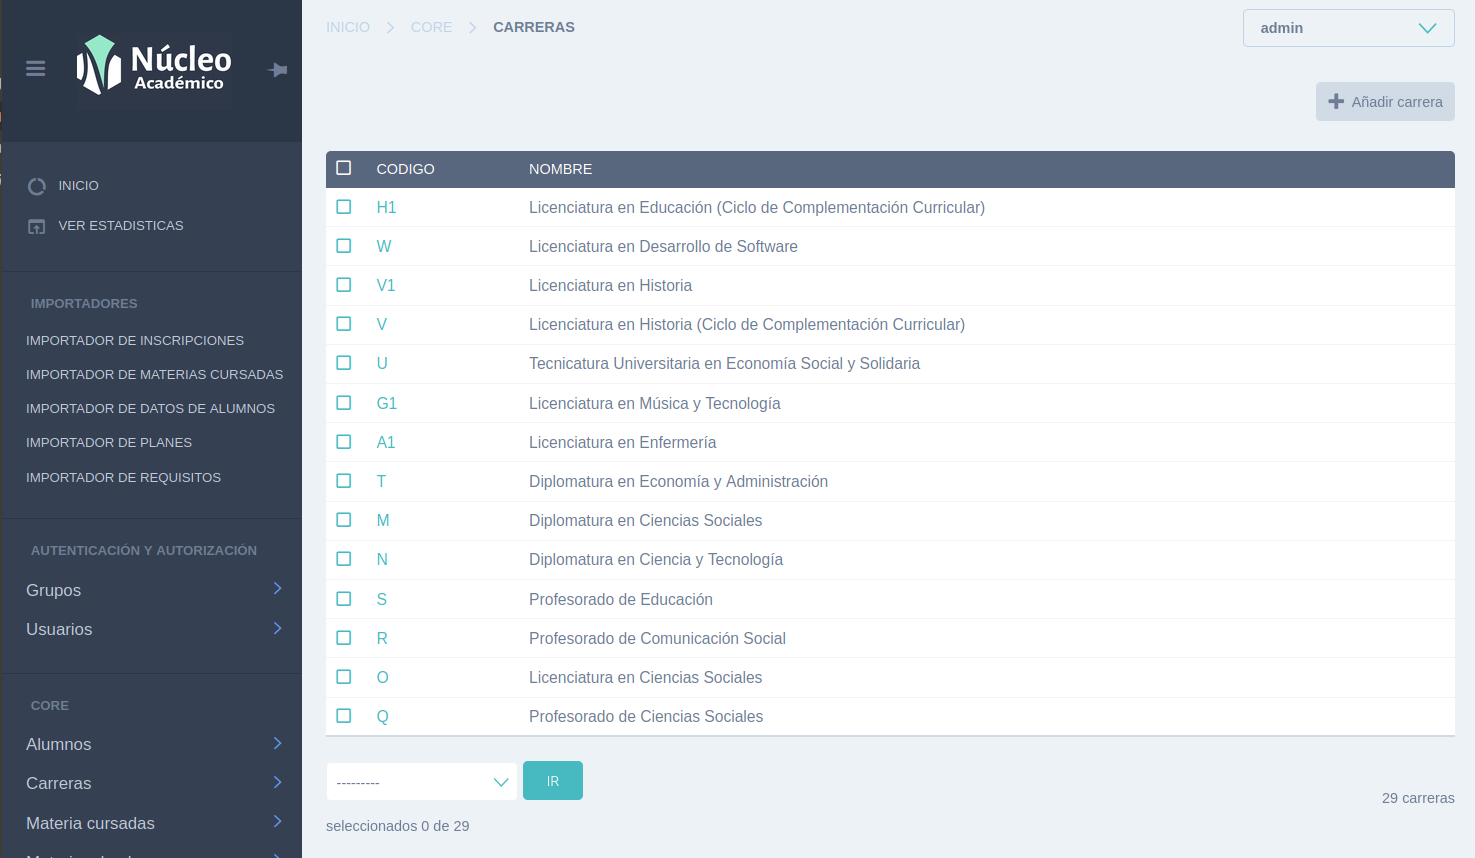
\includegraphics[scale=0.3]{images/nucleo/nucleo-list.png}
  \captionof{figure}{Pantalla de login}
  \label{fig:django}
\end{figure}

\subsubsection{Edicion}
\begin{figure}[h!]
  \centering
    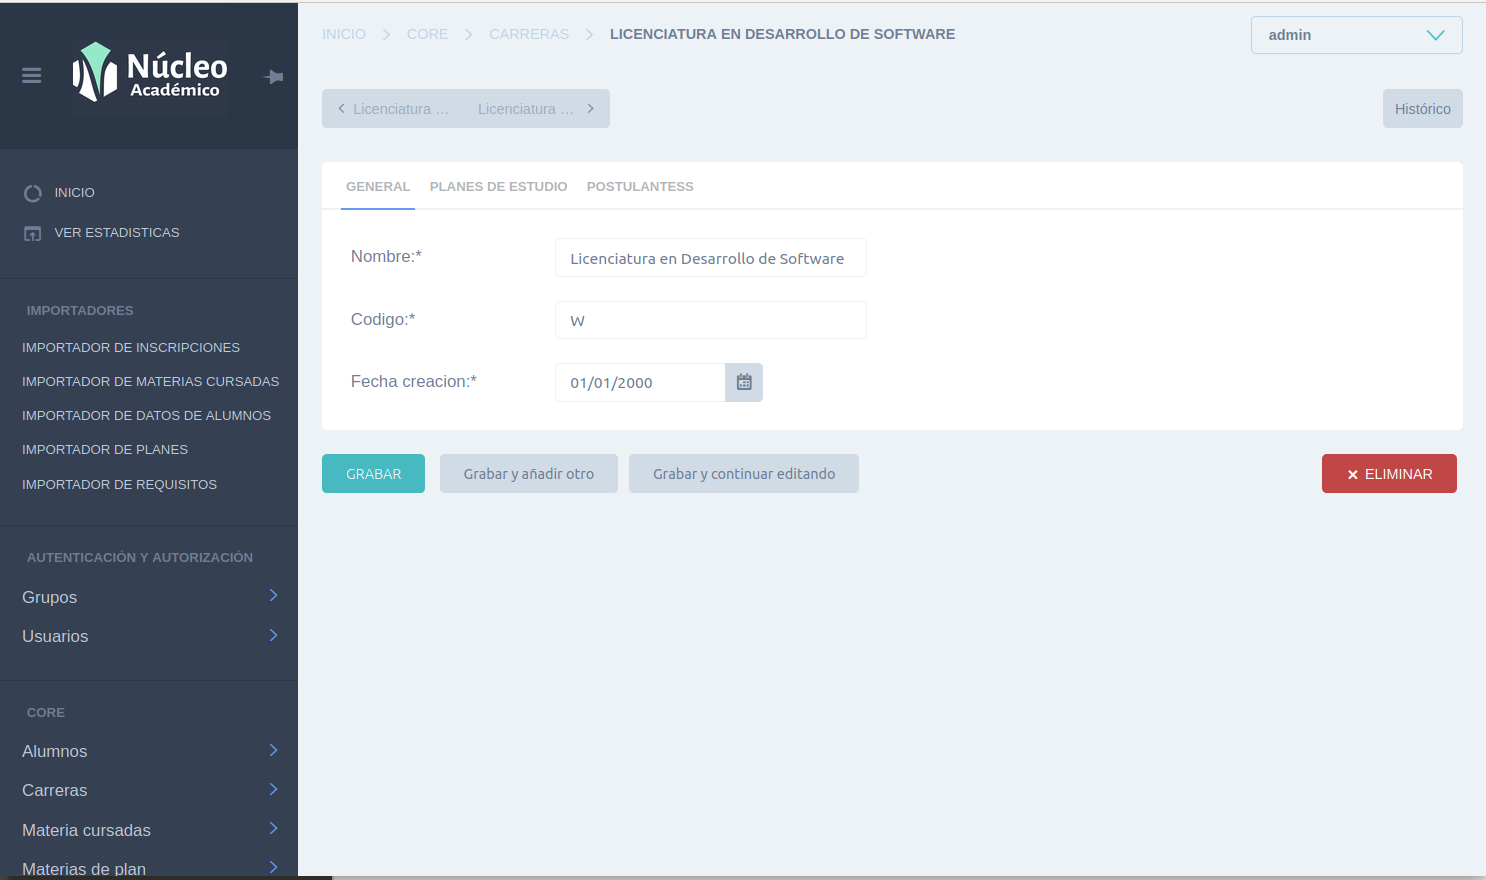
\includegraphics[scale=0.3]{images/nucleo/nucleo-edit.png}
  \captionof{figure}{Pantalla de login}
  \label{fig:django}
\end{figure}


















\section[Análisis de Datos]{Análisis de Datos}

\subsection{Tecnologías}

\subsection{API REST}

\subsection{}

\section[Visualización de los datos analizados]{Visualización de los datos analizados}

\subsection{Tecnologías}

